\documentclass{article}

\usepackage{graphicx}
\usepackage{hyperref}
\usepackage{tikz}
\usepackage{pgfplots}
\usepackage{multirow}
\usepackage{lipsum}
\usepackage{listings}
\usepackage{color}
\pgfplotsset{compat=1.16}
\pgfplotsset{width=10cm}


\author{Roșu Cristian-Mihai A2 \\ Manolache Mihai A2}
\title{HW3 Report - SAT}

\definecolor{dkgreen}{rgb}{0,0.6,0}
\definecolor{gray}{rgb}{0.5,0.5,0.5}
\definecolor{mauve}{rgb}{0.58,0,0.82}

\begin{document}

\lstset{frame=tb,
  language=C++,
  aboveskip=3mm,
  belowskip=3mm,
  showstringspaces=false,
  columns=flexible,
  basicstyle={\small\ttfamily},
  numbers=none,
  numberstyle=\tiny\color{gray},
  keywordstyle=\color{blue},
  commentstyle=\color{dkgreen},
  stringstyle=\color{mauve},
  breaklines=true,
  breakatwhitespace=true,
  tabsize=3
}

\maketitle

\begin{abstract}
This research paper analyzes the performance of a Genetic Algorithm against
the Simulated Annealing heuristic search algorithm applied on the 
\textit{Boolean Satisfiability Problem}(SAT).
\end{abstract}

\section{Introduction}
In logic and computer science, the Boolean satisfiability problem is the 
problem of determining if there exists an interpretation that satisfies a 
given Boolean formula. In other words, it asks whether the variables of a 
given Boolean formula can be consistently replaced by the values TRUE or 
FALSE in such a way that the formula evaluates to TRUE. If this is the case, 
the formula is called satisfiable. 
On the other hand, if no such assignment exists, the function expressed by 
the formula is FALSE for all possible variable assignments and the formula 
is unsatisfiable. \cite{wiki}

This paper aims to solve this problem by employing two different methods:

\begin{itemize}
    \item using a Genetic Algorithm
    \item using a Heuristic Search Method, specifically Simulated Annealing
\end{itemize}

It is expected that the Genetic Algorithm will yield the best results as it
generally outperforms the alternatives by a great margin. This assumption is
made in correlation with the results of the previous experiments.

\subsection{Motivation} 
The purpose of this work is to explore the capabilities of a Genetic Algorithm
against those of a heuristic search method.

In that sense, SAT was chosen due to its ease of implementation and of
understanding on a theoretical level. And as for the heuristic search method,
Simulated Annealing includes the abilities of alternatives such as Iterated
Hillclimbing while minimizing the danger of getting stuck in a local minima.
On top of that, it is equally easy to understand and implement. As such, it
is the perfect candidate. 


\section{Method}
The CNF formulas which represent the input of SAT are being parsed into
the algorithm from the DIMACS CNF format. \cite{dimacs}

The candidate solution for SAT has been represented identically in both
algorithms: a bitstring of length equal to the number of variables in the CNF
formula, the values of 1 and 0 representing TRUE and FALSE.

Since it would normally be impossible to compare SAT solutions, given the
fact that they either satisfy the formula or not, we choose to evaluate a 
solution based on its number of TRUE clauses.

\subsection{Genetic Algorithm}
The genetic operators used are mutation and crossover, and as for selection,
the \textbf{Roulette Wheel} method was used.

Since the solution is represented using a bitstring, the mutation and crossover
operators suffered no modification in their implementation in the case of SAT.

The selection, however, was modified slightly due to the method used to
calculate the fitness function. Specifically, the fitness of a cromozome
is equal to the number of satisfied clauses.

Following experiment results, a maximum \textbf{number of generations of 500} was chosen
since there was no real improvement in the solutions with bigger numbers.
As for the other values, a \textbf{mutation rate of 0.01} and a \textbf{crossover rate of 0.3}
were used.

\subsection{Simulated Annealing}
The function to maximize is derived from the input from the DIMACS CNF file,
and the solutions are compared based on the number of TRUE clauses. Apart
from that, the functionality of the algorithm remains the same.

In this case, a starting temperature of \textbf{100} was chosen with a
cooling rate of \textbf{0.999}.

\section{Experiment}
The experiment consists in running the Genetic Algorithm and Simulated
Annealing through 8 benchmarks of increasingly higher size \cite{benchmarks},
over 30 iterations in order to get a sample big enough to compare them by
looking at the minimum, maximum, average and standard deviation of the
solution produced, as well as the time needed to produce them.

The code for this can be found on Github \cite{github}.

\newpage

\section{Results}
Below are 8 tables corresponding to the experiment results for each benchmark,
and each benchmark has a different number of variables and clauses:

\begin{itemize}
    \item \textit{frb30-15-1.cnf} with \textbf{450 variables} and \textbf{19084 clauses}
    
    \begin{figure}[!htbp]
        \begin{tabular}{|c|c|c|c|c|c|}
        \hline
        \textbf{Method} & \textbf{Min} & \textbf{Max} & \textbf{Average} & \textbf{Sd} & \textbf{Time} \\ \hline
        Genetic Algorithm & 0 & 16513 & 14702.9756 & 436.2184 & 1702s \\ \hline
        Simulated Annealing & 13411 & 19077 & 18874.8352 & 696.4361 & 322s \\ \hline
        \end{tabular}
    \caption{frb30-15-1}
    \end{figure}

    Here, Simulated Annealing arrives at the better result, and faster, with
    a big margin compared to the Genetic Algorithm, being quite close to 19084.
    
    \item \textit{frb35-17-1.cnf} with \textbf{595 variables} and \textbf{29707 clauses}
    
    \begin{figure}[!htbp]
        \begin{tabular}{|c|c|c|c|c|c|}
        \hline
        \textbf{Method} & \textbf{Min} & \textbf{Max} & \textbf{Average} & \textbf{Sd} & \textbf{Time} \\ \hline
        Genetic Algorithm & 0 & 25595 & 22555.34106 & 546.1537 & 2246s \\ \hline
        Simulated Annealing & 21527 & 29696 & 29474.2374 & 833.5987 & 404s \\ \hline
        \end{tabular}
    \caption{frb35-17-1}
    \end{figure}

    In Figure 2, Simulate Annealing proves once again to be the better match.
    
    \item \textit{frb40-19-1.cnf} with \textbf{760 variables} and \textbf{43780 clauses}
    
    \begin{figure}[!htbp]
        \begin{tabular}{|c|c|c|c|c|c|}
        \hline
        \textbf{Method} & \textbf{Min} & \textbf{Max} & \textbf{Average} & \textbf{Sd} & \textbf{Time} \\ \hline
        Genetic Algorithm & 0 & 36655 & 33576.6104 & 788.1297 & 3632s \\ \hline
        Simulated Annealing & 7571 & 10673 & 10590.2980 & 312.9464 & 213s \\ \hline
        \end{tabular}
    \caption{frb40-19-1}
    \end{figure}

    From this point on, the Genetic Algorithm starts providing better and better
    results while Simulated Annealing drifts further and further away from the
    goal.
    
    \item \textit{frb45-21-1.cnf} with \textbf{945 variables} and \textbf{61855 clauses}
    
    \begin{figure}[!htbp]
        \begin{tabular}{|c|c|c|c|c|c|}
        \hline
        \textbf{Method} & \textbf{Min} & \textbf{Max} & \textbf{Average} & \textbf{Sd} & \textbf{Time} \\ \hline
        Genetic Algorithm & 0 & 51173 & 47209.8882 & 896.0659 & 4401s \\ \hline
        Simulated Annealing & 20707 & 28504 & 28225.1825 & 907.1837 & 411s \\ \hline
        \end{tabular}
    \caption{frb45-21-1}
    \end{figure}
    
    \newpage

    \item \textit{frb50-23-1.cnf} with \textbf{1150 variables} and \textbf{84508 clauses}
    
    \begin{figure}[!htbp]
        \begin{tabular}{|c|c|c|c|c|c|}
        \hline
        \textbf{Method} & \textbf{Min} & \textbf{Max} & \textbf{Average} & \textbf{Sd} & \textbf{Time} \\ \hline
        Genetic Algorithm & 0 & 69589 & 64072.9148 & 1145.0336 & 6672s \\ \hline
        Simulated Annealing & 12797 & 18012 & 17767.8844 & 642.8460 & 347s \\ \hline
        \end{tabular}
    \caption{frb50-23-1}
    \end{figure}
    
    \item \textit{frb53-24-1.cnf} with \textbf{1270 variables} and \textbf{98921 clauses}
    
    \begin{figure}[!htbp]
        \begin{tabular}{|c|c|c|c|c|c|}
        \hline
        \textbf{Method} & \textbf{Min} & \textbf{Max} & \textbf{Average} & \textbf{Sd} & \textbf{Time} \\ \hline
        Genetic Algorithm & 0 & 81104 & 74952.3112 & 1450.3403 & 7772s \\ \hline
        Simulated Annealing & 23473 & 32215 & 31518.4353 & 1140.3133 & 646s \\ \hline
        \end{tabular}
    \caption{frb53-24-1}
    \end{figure}
    
    \item \textit{frb56-25-1.cnf} with \textbf{1400 variables} and \textbf{114668 clauses}
    
    \begin{figure}[!htbp]
        \begin{tabular}{|c|c|c|c|c|c|}
        \hline
        \textbf{Method} & \textbf{Min} & \textbf{Max} & \textbf{Average} & \textbf{Sd} & \textbf{Time} \\ \hline
        Genetic Algorithm & 0 & 94095 & 87121.6556 & 1430.3610 & 8763s \\ \hline
        Simulated Annealing & 10503 & 14879 & 14660.4627 & 532.6347 & 297s \\ \hline
        \end{tabular}
    \caption{frb56-25-1}
    \end{figure}
    
    \item \textit{frb59-26-1.cnf} with \textbf{1534 variables} and \textbf{132295 clauses}

    \begin{figure}[!htbp]
        \begin{tabular}{|c|c|c|c|c|c|}
        \hline
        \textbf{Method} & \textbf{Min} & \textbf{Max} & \textbf{Average} & \textbf{Sd} & \textbf{Time} \\ \hline
        Genetic Algorithm & 0 & 107362 & 100082.6476 & 1627.0163 & 9914s \\ \hline
        Simulated Annealing & 23400 & 31878 & 31087.7561 & 1160.8581 & 559s \\ \hline
        \end{tabular}
    \caption{frb59-26-1}
    \end{figure}

\end{itemize}

And below are 2 pairs of graphs highlighting the evolution of the best solution
produced by each of the 2 methods, which coresponds to the maximum value at
each iteration, in the case of Simulated Annealing, and at each generation,
in the case of the Genetic Algorithm.

The first pair showcases their behaviour on a small number of variables and
clauses (frb30-15-1.cnf in Figure 1), while the second pair presents a
benchmark with a significantly bigger number of variables and clauses 
(frb59-26-1.cnf in Figure 8).

The Y axis represents the range of values found and the X axis represents
the temperature's evolution, specifically the number of times it took for it
to sufficiently cool down, in the case of Simulated Annealing, and it 
represents the generation's number in the case of the Genetic Algorithm.

\begin{figure}[!htbp]
    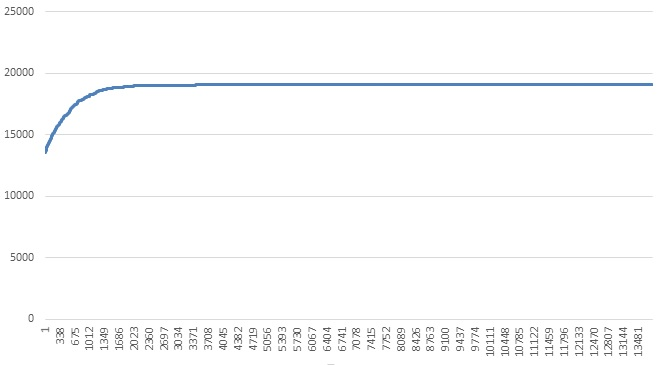
\includegraphics[scale=0.6]{SAsmall.jpg}
    \caption{SA frb30-15-1.cnf}
\end{figure}

\begin{figure}[!htbp]
    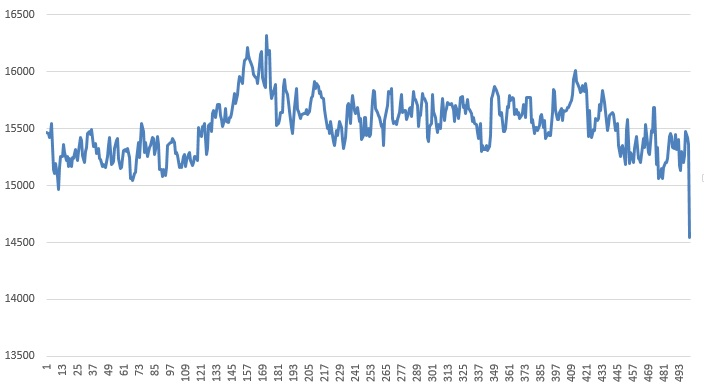
\includegraphics[scale=0.6]{GAsmall.jpg}
    \caption{GA frb30-15-1.cnf}
\end{figure}

\begin{figure}[!htbp]
    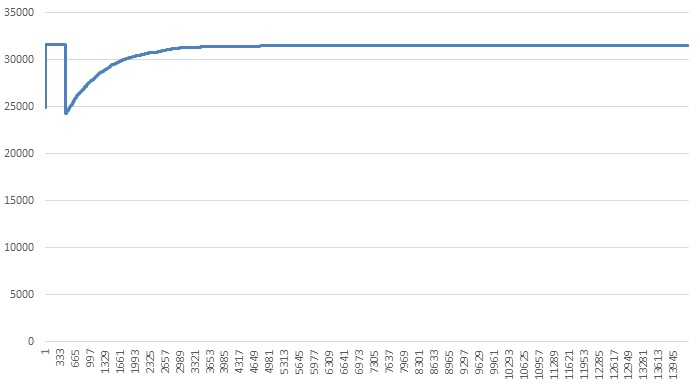
\includegraphics[scale=0.6]{SAbig.jpg}
    \caption{SA frb59-26-1.cnf}
\end{figure}

\begin{figure}[!htbp]
    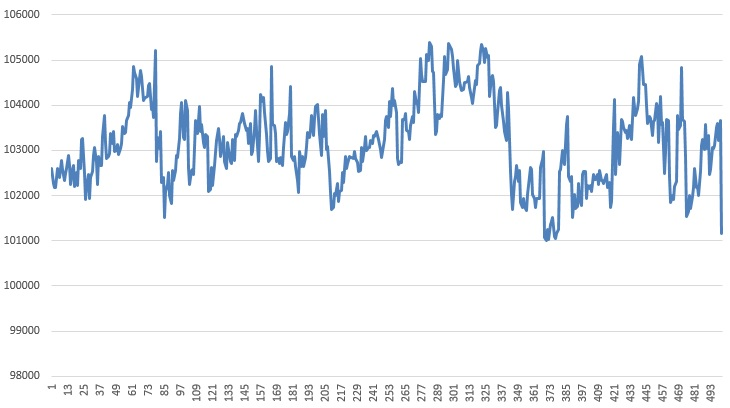
\includegraphics[scale=0.6]{GAbig.jpg}
    \caption{GA frb59-26-1.cnf}
\end{figure}

\newpage

\section{Conclusions}
Seeing the results, Simulated Annealing outperforms the Genetic Algorithm
when it comes to smaller samples. It arrives at a near-perfect solution in
a very short time and with quite a margin, as seen in Figure 1 and 2.

However, from Figure 3 onwards, the Genetic Algorithm consistently outperforms
Simulated Annealing with bigger and bigger differences.

From this, we can draw the conclusion that the Genetic Algorithm is
the better alternative to this problem as it scales upwards.

It is worth mentioning that both methods could be improved in an unforeseen
way that could potentially produce better results.

\begin{thebibliography}{9}

\bibitem{wiki}
    Wikipedia page for SAT \\
    \url{https://en.wikipedia.org/wiki/Boolean_satisfiability_problem}

\bibitem{dimacs}
    DIMACS CNF format definition \\
    \url{https://logic.pdmi.ras.ru/~basolver/dimacs.html}

\bibitem{benchmarks}
    Site with benchmarks used \\
    \url{http://sites.nlsde.buaa.edu.cn/~kexu/benchmarks/benchmarks.htm}

\bibitem{github}
    Github repository for the project \\
    \url{https://github.com/Nenma/ga-hw3}

\end{thebibliography}
\end{document}